
\documentclass[12pt]{amsart}
\usepackage{geometry} 
\usepackage{graphicx}
\usepackage{subcaption}
\usepackage{dirtytalk}
\usepackage[spanish, activeacute]{babel}
\usepackage{hyperref}
\hypersetup{
    colorlinks,
    citecolor=black,
    filecolor=black,
    linkcolor=blue,
    urlcolor=black
}
\geometry{a4paper} 



\begin{document}

\begin{titlepage}
	\begin{center}	
	\huge{\bfseries{Manual de Usuario}}\\
	[0.1cm]
	\line(1,0){300}\\\\
	\huge{\bfseries{Programaci\'on orientada a objetos}}
	\textsc{\small{Emilio Cant\'on}}\
	\textsc{\small{Roberto Gervacio}}\
	\textsc{\small{Yann Le Lorier}}
	\begin{figure}
		
\includegraphics[width=\linewidth]{images/Tec.jpg}
	\end{figure}
	
	\end{center}

\end{titlepage}

\tableofcontents

\section{Introducci'on}
\hspace{10mm}Con el regreso de las modas noventeras, decidimos implementar un tamagotchi que permite a los nost'algicos como nosotros de revivir experiencias de la infancia, por medio de un programa de Java, el cual se controla por completo con las flechas del teclado.

\section{La interfaz de inicio}
\hspace{10mm}El programa empieza con una pantalla de bienvenida, que permite al usuario de escoger entre varias personalidades de tamagotchi (imagen \ref{welcome})
\subsection{Perfiles de personajes}
Para pasar entre los diferentes personajes, simplemente pasar entre las flechas de la derecha o izquierda, y para seleccionar una en espec'ifico, oprimir la flecha superior. (imagen \ref{welcome})\\
Existen varios perfiles que afectan el comportamiento de su nuevo tamagotchi, que lo vuelven m'as propenso a querer dormir, comer, entre otras actividades que ser'an definidas a continuaci'on.

\begin{itemize}
\item El personaje de \say{Player} es un personaje que tiene la necesidad de jugar m'as de lo normal (imagen \ref{player}).
\item El personaje de \say{Lovely} es uno que requiere de extra atenci'on, es decir m'as tiempo de juego con 'el, y se apega f'acilmente a su due\~no al hacer actividades como comer o jugar (imagen \ref{lovely}).
\item El personaje de \say{Slugabed} es simplemente muy flojo, lo cual lo forza a pedirle a su due\~no de descansar m'as de lo normal (imagen \ref{slugabed}).
\item El personaje de \say{Delicate} es para los entusiastas de las mascotas m'as experimentados, ya que se enferma f'acilmente, ya sea con la comida, o por el simple paso del tiempo (imagen \ref{delicate}) .
\end{itemize}

\begin{figure}
	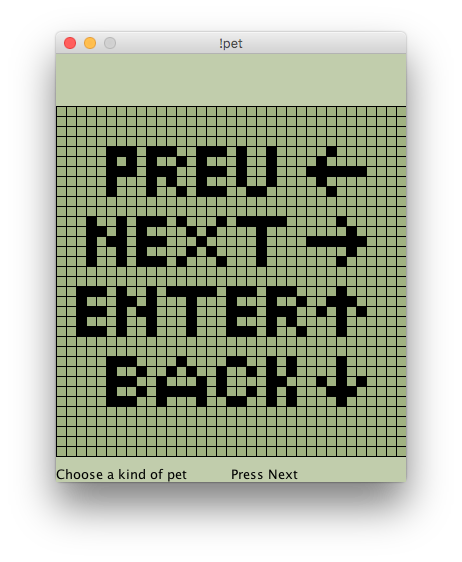
\includegraphics[width=5.0cm]{images/Welcome.jpg}
	\caption{Las opciones otorgadas al usuario para la selecci'on de un personaje.}
	\label{welcome}
\end{figure} 

\begin{figure}
	\begin{subfigure}[b]{4cm}
		\centering
		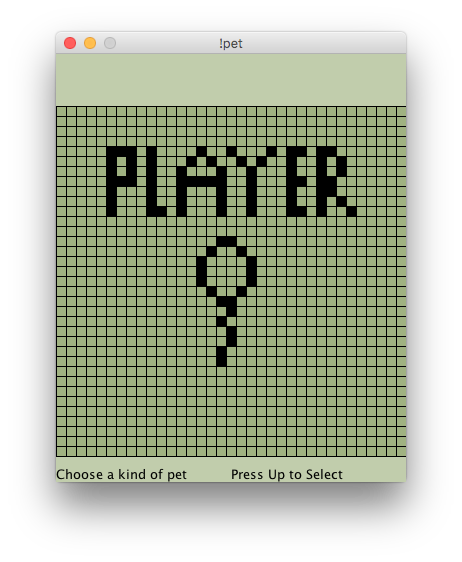
\includegraphics[width=4cm]{images/Player.jpg}
		\caption{Personaje \say{Player}}
		\label{player}
	\end{subfigure}
	\begin{subfigure}[b]{4cm}
		\centering
		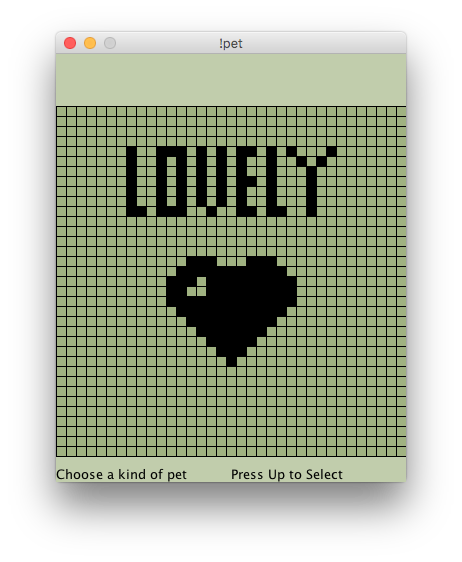
\includegraphics[width=4cm]{images/Lovely.jpg}
		\caption{Personaje \say{Lovely}}
		\label{lovely}
	\end{subfigure}

	\begin{subfigure}[b]{4cm}
		\centering
		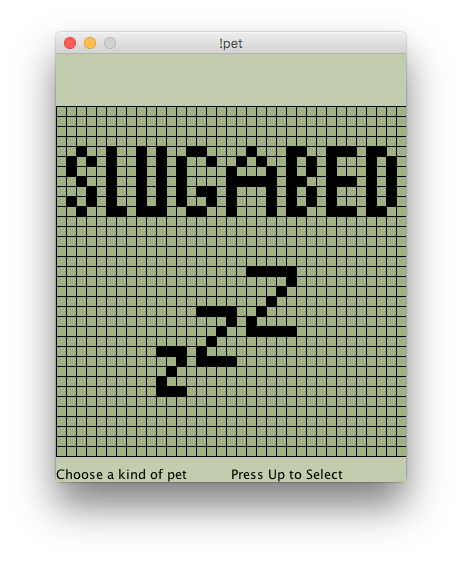
\includegraphics[width=4.0cm]{images/Slugabed.jpg}
		\caption{Personaje \say{Slugabed}}
		\label{slugabed}
	\end{subfigure}
	\begin{subfigure}[b]{4cm}
		\centering
		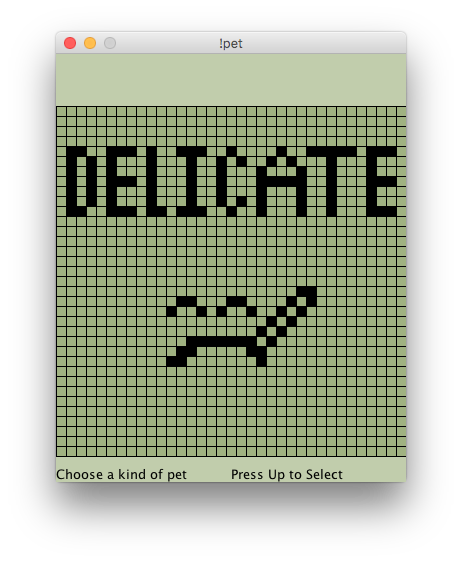
\includegraphics[width=4cm]{images/Delicate.jpg}
		\caption{Personaje \say{Delicate}}
		\label{delicate}
	\end{subfigure}
		\caption{Personajes disponibles en la pantalla de inicio}
		\label{personajes}
\end{figure}

\section{La pantalla de juego}
\hspace{10mm}Una vez seleccionado el perfil deseado para jugar, una ventana aparecer'a pregunt'andole al usuario el nombre de la mascota, s'olo ingresar el nombre y presionar \textit{retorno}.
\begin{figure}
	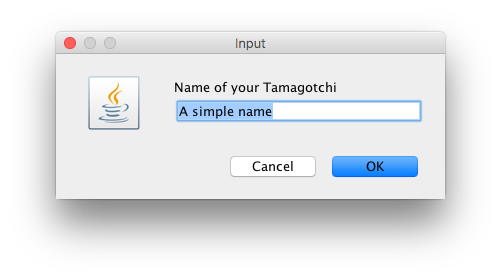
\includegraphics[width=7.0cm]{images/Name.jpg}
	\caption{Ingresar el nombre en el Pop-up}
	\label{name}
\end{figure}

\subsection{Los botones}
Al llegar a la pantalla de juego, es necesario estar familiarizado con los botones y con las exigencias del personaje.\\
En la imagen \ref{botones}, tenemos un conjunto de botones en la parte superior de la interfaz que nos permiten interactuar con la mascota, a los cuales se pueden acceder por medio de las flechas del teclado. De izquierda a derecha, 'estas son las actividades representadas por los botones:\\
\begin{itemize}
	\item Comer
	\item Dormir
	\item Jugar
	\item Sanar
	\item Ba\~nar
	\item Rega\~nar
	\item Mostrar el estado general de la mascota
	\item Controles
\end{itemize}

\begin{figure}
	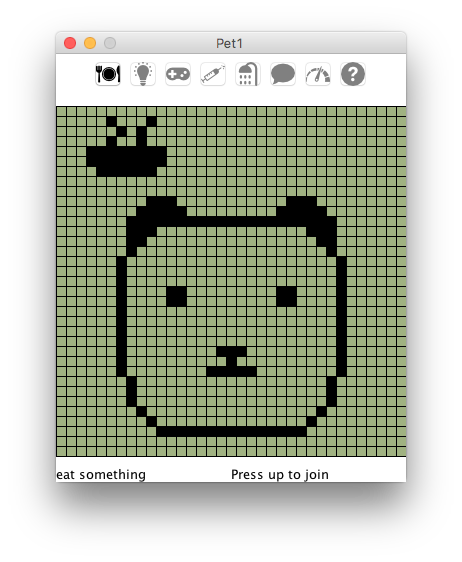
\includegraphics[width=7cm]{images/Botones.jpg}
	\caption{interfaz principal de juego}
	\label{botones}
\end{figure}

\subsection{Conociendo las exigencias de tu nueva mascota}
Por medio de los dibujos que aparecen encima de la mascota, es posible saber qu'e es lo que quiere:\\

\subsubsection{Comer}
En el ejemplo de la imagen \ref{botones}, podemos ver un plato de sopa, indic'andonos que nuestra mascota desea comer. Con la ayuda de las flechas del teclado, acceder a la actividad correspondiente para comer.

\subsubsection{Dormir}
En el ejemplo de la figura \ref{sleepy}, podemos ver que el 'icono dibujado por encima de nuestra mascota son unas \say{Z}, indic'andonos que quiere dormir.

\subsubsection{Jugar}
La figura \ref{playful} muestra que la mascota quiere jugar, requiere de atenci'on, por lo cual el dibujo en cuesti'on es \say{!!}.

\subsubsection{Enfermo}
La figura \ref{sick} muestra que tu mascota no se siente bien y que necesita que la sanes. Operando las flechas del teclado, accede al 'icono de la jeringa y oprime la flecha superior.

\subsubsection{Triste}
Independientemente de la edad de tu mascota, se puede llegar a sentir triste, por lo que debes de darle atenci'on o comida, para que no se sienta triste (imagen \ref{sad}).

\subsubsection{Latoso}
Si tu mascota se pone de latosa, debes de hablar con ella. Puedes saber si est'a siendo mal portado por que le aparecen unos cuernos. Habla con 'el con el 'icono de la burbuja.


\begin{figure}
	\begin{subfigure}[b]{5cm}
	\centering
	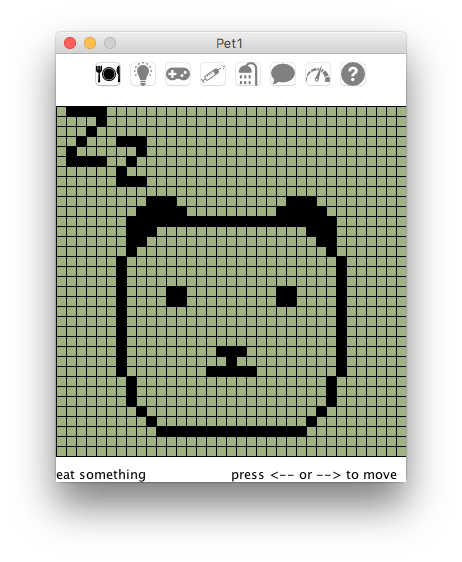
\includegraphics[width=6cm]{images/Sleepy.jpg}
	\caption{Mascota con sue\~no}
	\label{sleepy}
	\end{subfigure}
	\begin{subfigure}[b]{5cm}
	\centering
	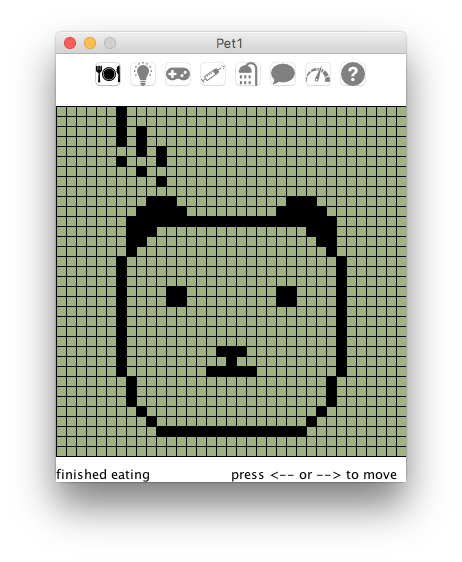
\includegraphics[width=6cm]{images/Playful.jpg}
	\caption{La mascota quiere jugar}
	\label{playful}
	\end{subfigure}

	\begin{subfigure}[b]{5cm}
	\centering
	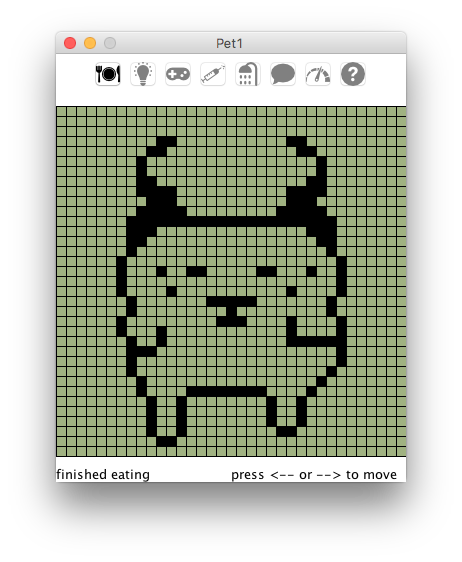
\includegraphics[width=6cm]{images/Talk.jpg}
	\caption{Necesita disciplina}
	\label{talk}
	\end{subfigure}

	\begin{subfigure}[b]{5cm}
	\centering
	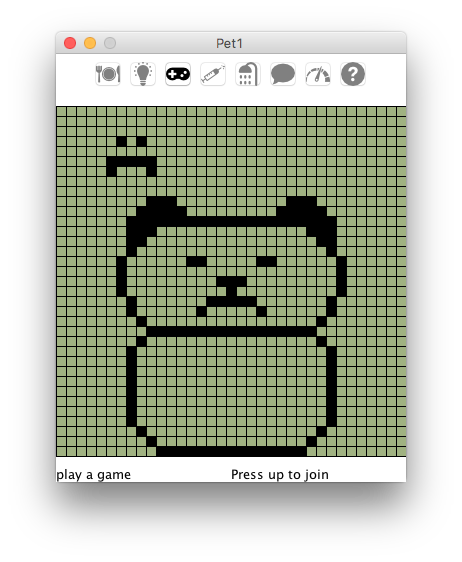
\includegraphics[width=6cm]{images/Sad.jpg}
	\caption{La mascota est\'a triste}
	\label{sad}
	\end{subfigure}
	\begin{subfigure}[b]{5cm}
	\centering
	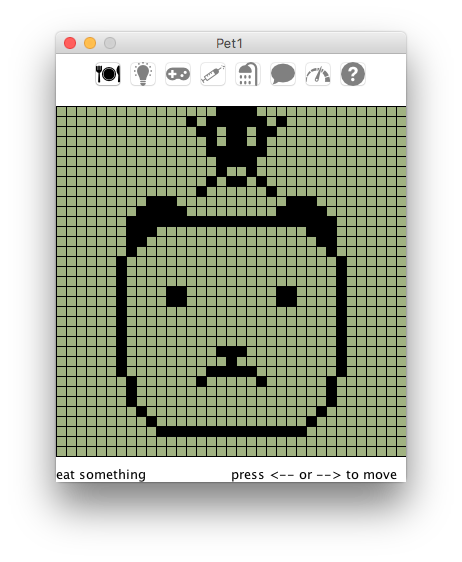
\includegraphics[width=6cm]{images/Sick.jpg}
	\caption{La mascota est\'a enferma}
	\label{sick}
	\end{subfigure}
	\caption{Las necesidades de tu mascota}
\end{figure}

\end{document}
